\chapter[Planejamento]{Planejamento}
\label{cap:planejamento}

Antes de iniciar o desenvolvimento do projeto, foram especificados os recursos necessários para a montagem do sistema e sua utilização.
Esta seção descreve a escolha do equipamento e o projeto inicial do sistema.

\section[Escolha do equipamento]{Escolha do equipamento}
\label{sec:escolhaEquipamento}

Para o desenvolvimento do projeto, foram disponibilizados, pela instituição CEFET-MG, dois manipuladores robóticos e diversos dispositivos que podem ser utilizados para seu controle.
A partir desse equipamento, e de outros disponíveis no mercado, foi decidido como o projeto seria realizado.
Os equipamentos utilizados para o projeto estão descritos a seguir:

\subsection[Manipuladores]{Manipuladores}

Os principais elementos deste trabalho são os manipuladores robóticos, portanto foi feito inicialmente um estudo sobre seu funcionamento e sobre como seu controle pode ser realizado para movimentar as peças de xadrez.

Foi disponibilizado um manipulador robótico de modelo Mentor de cor preta, conforme a figura \ref{fig:fotoManipuladorMentor}, e um manipulador de modelo RD5NT de cor azul, conforme a figura \ref{fig:fotoManipuladorRD5NT}.
Eles possuem diversas juntas movimentadas por motores de corrente contínua, e permitem que o manipulador funcione de forma similar a um braço humano.
Além disso, cada junta possui um potenciômetro que indica a posição atual do eixo, por meio de um sinal analógico.

O manipulador Mentor apresenta 5 graus de liberdade e uma garra que pode ser utilizada para pegar e soltar objetos.
Além disso, ele possui caixas de redução em seus motores, o que permite que ele mantenha sua posição mesmo após o desligamento dos motores.
Suas dimensões e faixas de movimento são apresentadas na tabela \ref{tab:caracteristicasManipuladorMentor} \cite{mentor_forward_kinematics}.

Já o manipulador RD5NT possui apenas 4 graus de liberdade e uma garra.
Além de não possuir caixa de redução em seus motores, ele utiliza molas em alguns eixos, o que faz com que perca sua posição quando os motores são desligados.
Portanto, seu controle deve ser realizado de forma contínua para que permaneça na posição desejada.
Suas dimensões e faixas de movimento são apresentadas na tabela \ref{tab:caracteristicasManipuladorRD5NT} \cite{controle_neural_robo}.

\begin{table}
    \centering
    \caption{Características do manipulador robótico Mentor}
    \label{tab:caracteristicasManipuladorMentor}
    \begin{tabular}{|l|l|l|}
        \hline
        \textbf{Eixo} & \textbf{Movimento angular (graus)} & \textbf{Comprimento (mm)} \\ \hline
        \textbf{Eixo 0 (Torso)}                    & 210 & 185 \\ \hline
        \textbf{Eixo 1 (Ombro)}                    & 180 & 165 \\ \hline
        \textbf{Eixo 2 (Cotovelo)}                 & 230 & 150 \\ \hline
        \textbf{Eixo 3 (Esquerdo do Pulso)}        & 320 & 0 \\ \hline
        \textbf{Eixo 4 (Direito do Pulso)}         & 320 & 0 \\ \hline
        \textbf{Pulso \textit{Pitch}}              & 140 & - \\ \hline
        \textbf{Pulso \textit{Roll}}               & 320 & - \\ \hline
    \end{tabular}
\end{table}

\begin{table}
    \centering
    \caption{Características do manipulador robótico RD5NT}
    \label{tab:caracteristicasManipuladorRD5NT}
    \begin{tabular}{|l|l|l|}
        \hline
        \textbf{Eixo} & \textbf{Movimento angular (graus)} & \textbf{Comprimento (mm)} \\ \hline
        \textbf{Eixo 0 (Torso)}            & 293 & 110 \\ \hline
        \textbf{Eixo 1 (Ombro)}            & 107 & 120 \\ \hline
        \textbf{Eixo 2 (Cotovelo)}         & 284 & 160 \\ \hline
        \textbf{Eixo 3 (Pulso)}            & 360 & 0 \\ \hline
    \end{tabular}
\end{table}

\begin{figure}[H]
    \begin{minipage}{.5\textwidth}
        \centering
        \caption{Manipulador robótico Mentor}
        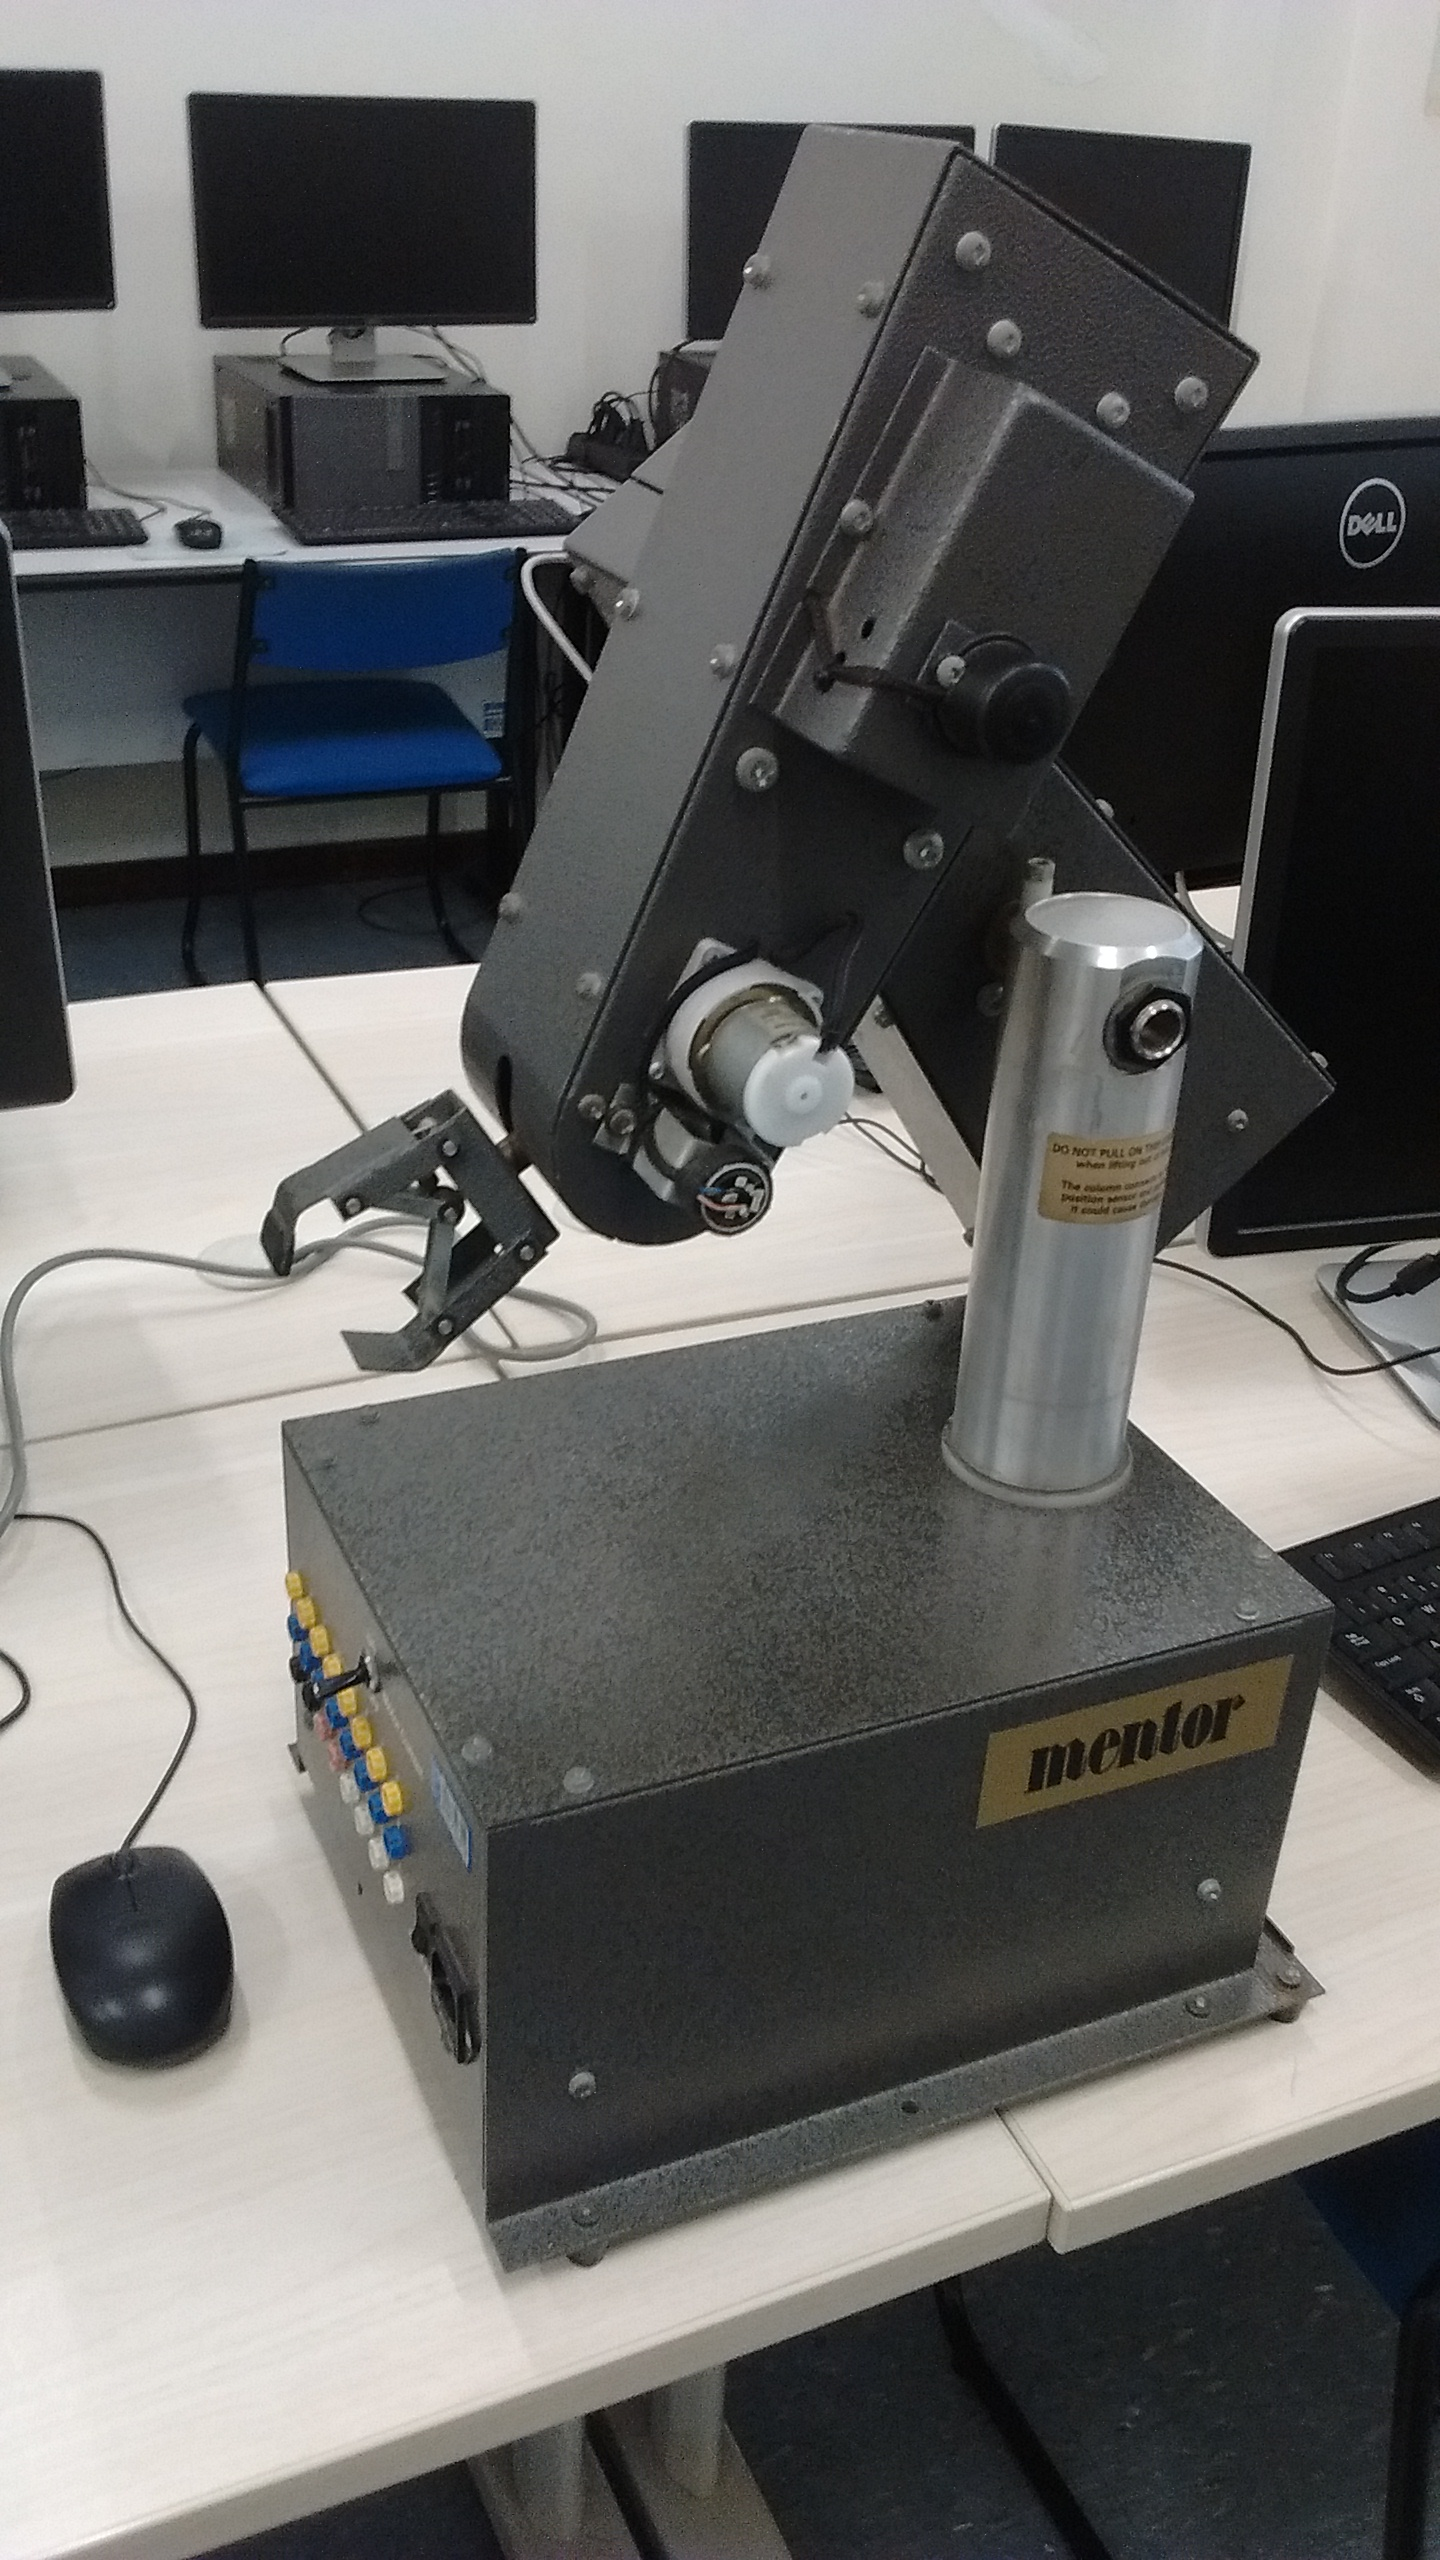
\includegraphics[keepaspectratio=true, width=0.9\linewidth]
            {img/foto-manipulador-preto.jpg}
        \fonte{http://arquivo.eng.br/robotica}
        \label{fig:fotoManipuladorMentor}
    \end{minipage}
    \begin{minipage}{.5\textwidth}
        \centering
        \caption{Manipulador robótico RD5NT}
        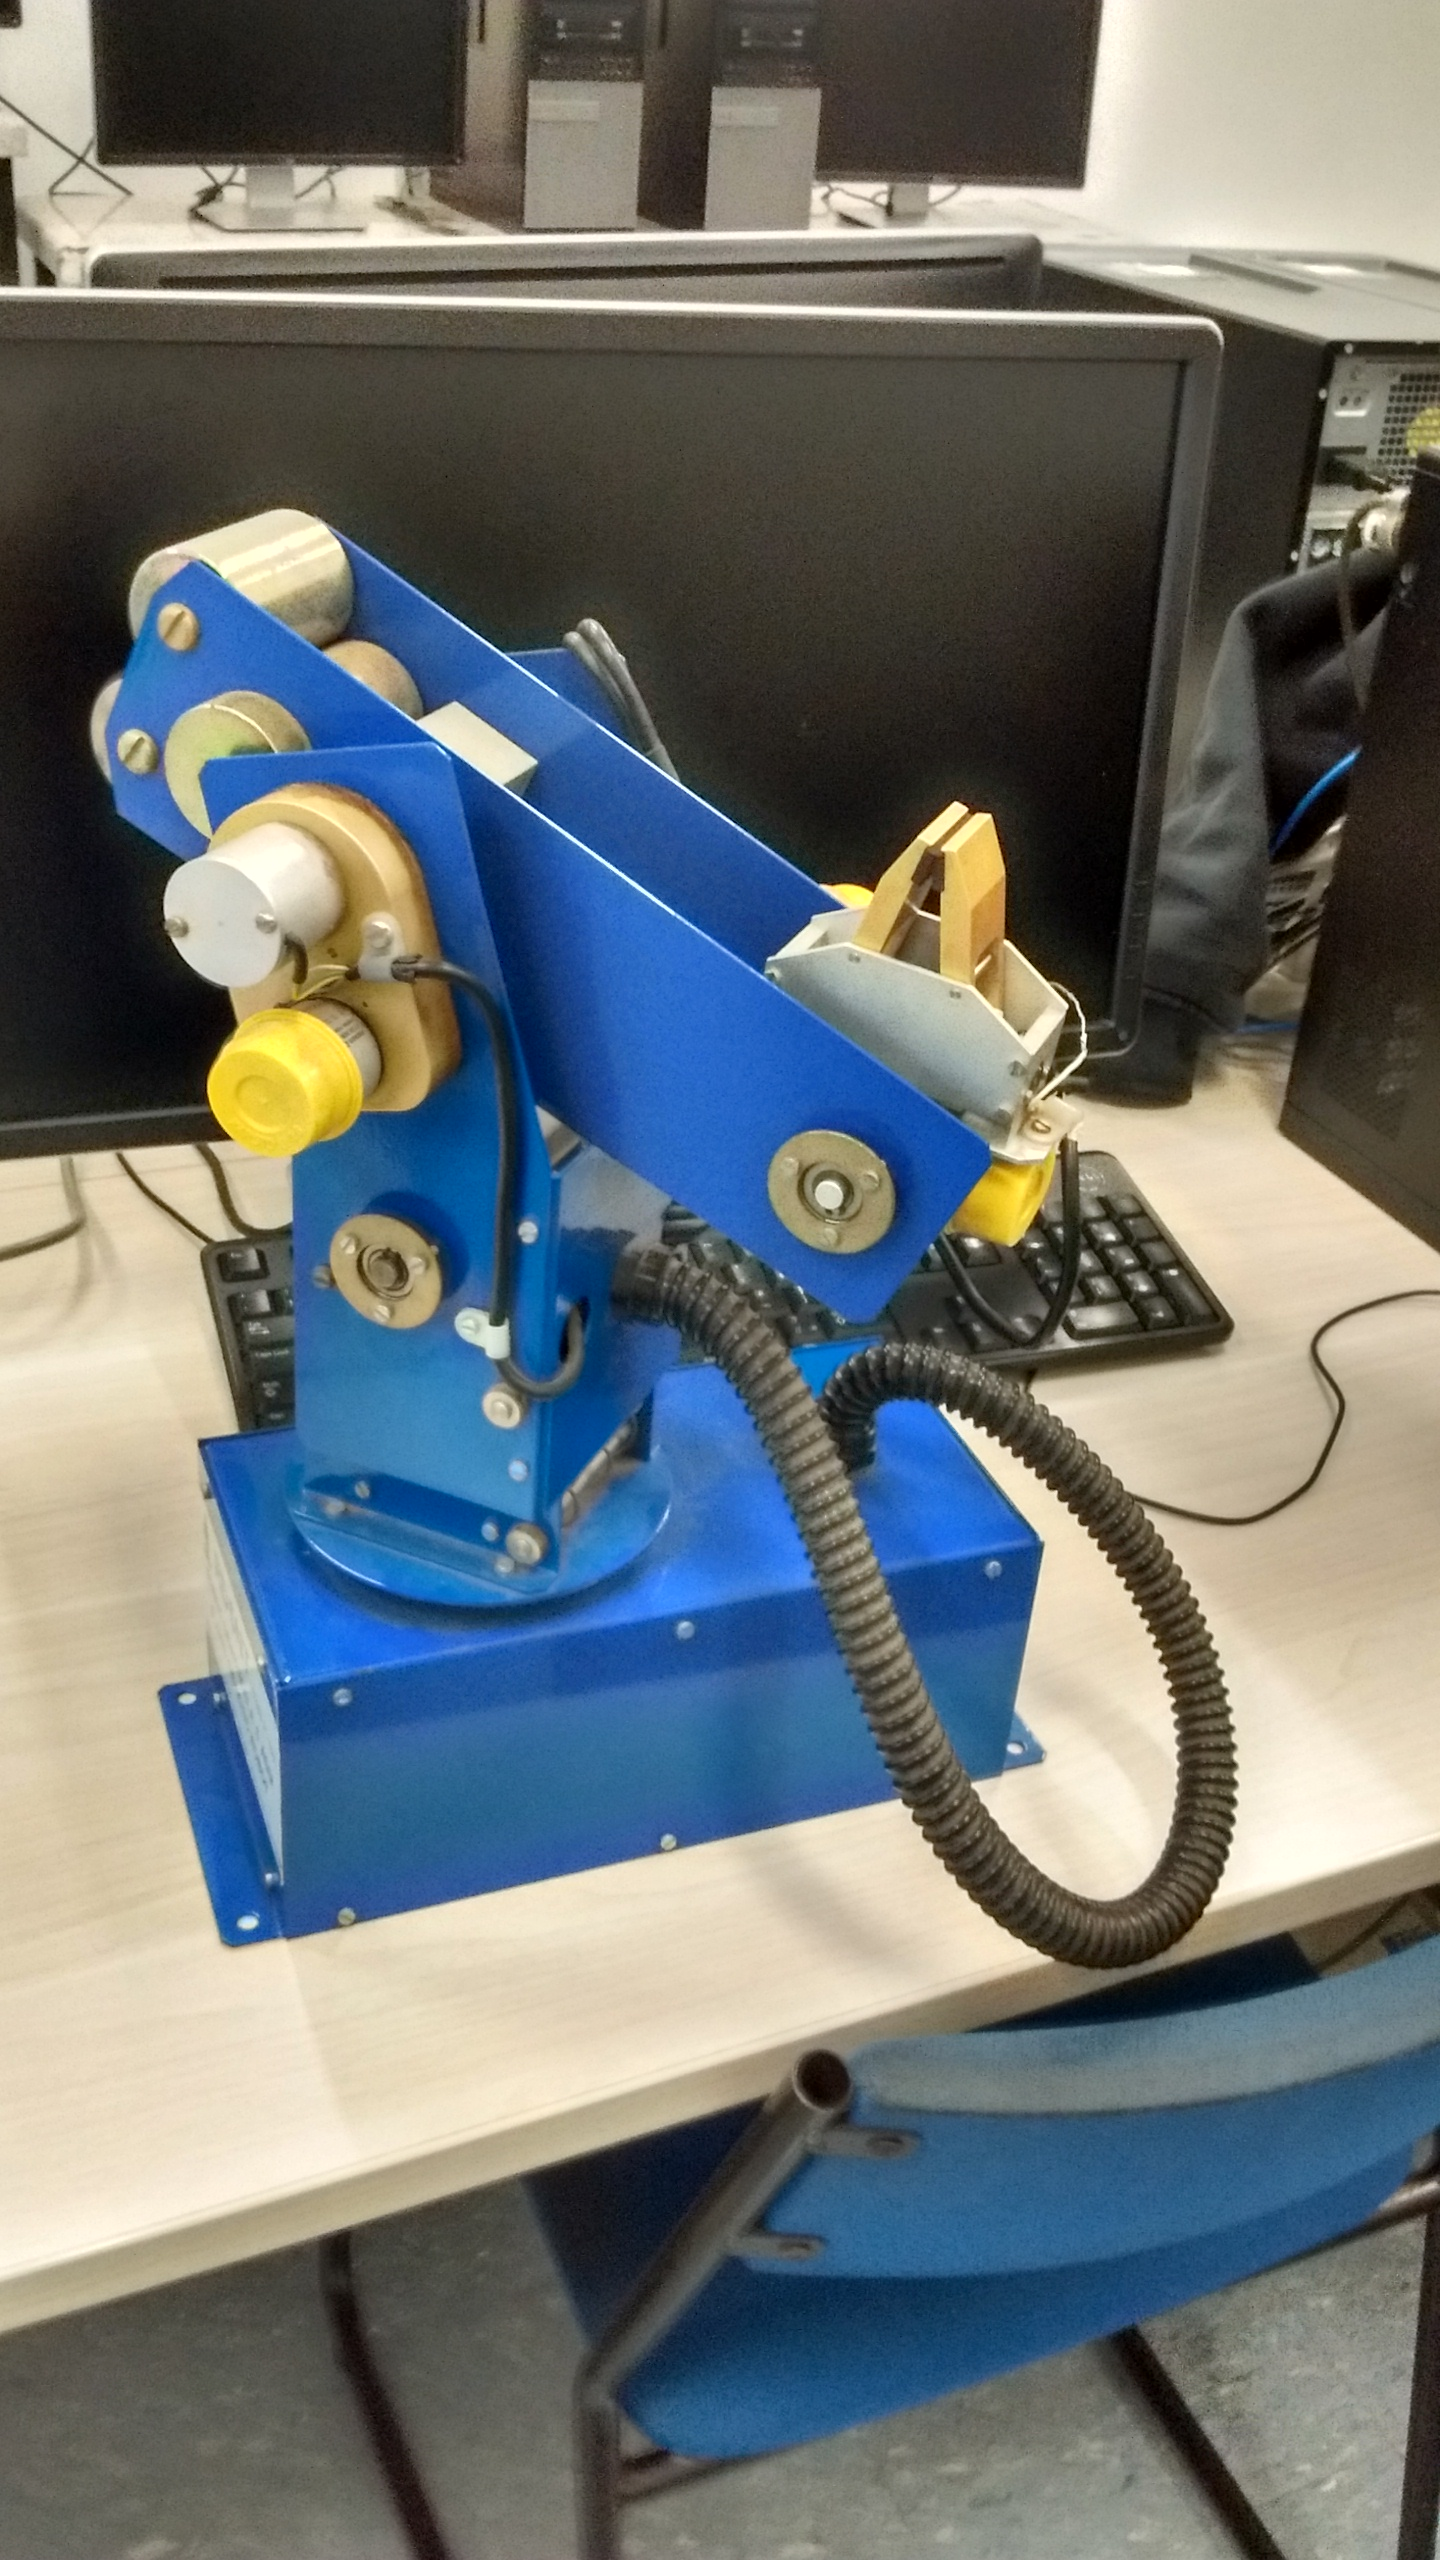
\includegraphics[keepaspectratio=true, width=0.9\linewidth]
            {img/foto-manipulador-RD5NT.jpg}
        \fonte{http://arquivo.eng.br/robotica}
        \label{fig:fotoManipuladorRD5NT}
    \end{minipage}%
\end{figure}

Foi decidido utilizar o manipulador de modelo RD5NT para o projeto, pois ele possui menos graus de liberdade na sua garra, o que facilita a implementação do algoritmo de controle.
Além disso, ele possui uma garra de tamanho adequado para pegar as peças de xadrez sem derrubar as outras peças do tabuleiro.
Apesar de não possuir caixa de redução em seus motores, isso não é um problema, pois o controle do manipulador será realizado de forma contínua.

\subsection[Manete para o jogador]{Manete para o jogador}
\label{sub:maneteJogador}

Para que o jogador possa interagir com o manipulador, foi decidido utilizar uma manete de modelo \textit{batpad}, que possui dois \textit{joysticks}, conforme a figura \ref{fig:fotoManeteJogador}.

Esses \textit{joysticks} devem ser alimentados com 3.3V ou 5V e permitem a leitura de posição em duas dimensões, através de sinais analógicos.
Eles também possuem um botão que envia um sinal digital ao ser pressionado.

\begin{figure}[H]
    \centering
    \caption{Manete para o jogador}
    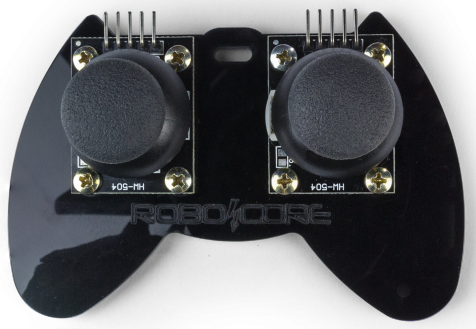
\includegraphics[keepaspectratio=true, width=0.5\textwidth]
    	{img/foto-controle-jogadores.png}
    \fonte{https://www.robocore.net/acessorios-robocore/controle-batpad}
    \label{fig:fotoManeteJogador}
\end{figure}

\subsection[Microcontrolador]{Microcontrolador}
\label{sub:microcontrolador}

Para realizar a integração entre a manete e o manipulador, foi decidido utilizar um microcontrolador ESP32, conforme a figura \ref{fig:fotoESP32}.
Esse microcontrolador possui um \textit{clock} de 240MHz, 4MB de memória \textit{flash} e 320KB de memória \textit{RAM}.
Ele apresenta ao todo 34 pinos que podem ser utilizados como entrada ou saída, e suporta sinais analógicos e digitais \cite{esp32_datasheet}.

Para permitir o controle manual do manipulador robótico, o microcontrolador faz a leitura dos sinais analógicos e digitais provenientes da manete com alguns de seus 18 canais de \textit{ADC} (\textit{Analog to Digital Converter})[Conversor Analógico Digital].
E para permitir o controle automático, ele recebe sinais de controle de um computador através de um cabo USB.
A partir desses sinais, o ESP32 realiza o cálculo das posições desejadas de cada junta do manipulador.

Para controlar os motores, o microcontrolador primeiramente faz a leitura dos sinais analógicos provenientes dos potenciômetros de cada junta.
A partir desses sinais, é possível determinar a posição atual de cada junta.
Com base na posição atual e na posição desejada, o microcontrolador envia um sinal de controle para os motores do manipulador robótico.

Os sinais de controle são digitais do tipo \textit{PWM} (\textit{Pulse Width Modulation}), que variam de 0V a 3.3V e possibilitam o controle da velocidade de rotação dos motores através da variação da tensão média.
Valores maiores de \textit{Duty Cycle} [Ciclo de Trabalho] resultam em maior velocidade de rotação do motor, pois o sinal permanece em nível alto por um período maior de tempo.
Por outro lado, valores menores de \textit{Duty Cycle} resultam em menor velocidade de rotação do motor, pois o sinal permanece em nível alto por um período menor de tempo.
Para definir o sentido de rotação do motor, foi utilizado um sinal digital que indica se ele deve girar no sentido horário ou anti-horário.

\begin{figure}[H]
    \centering
    \caption{Largura do pulso do sinal de controle}
    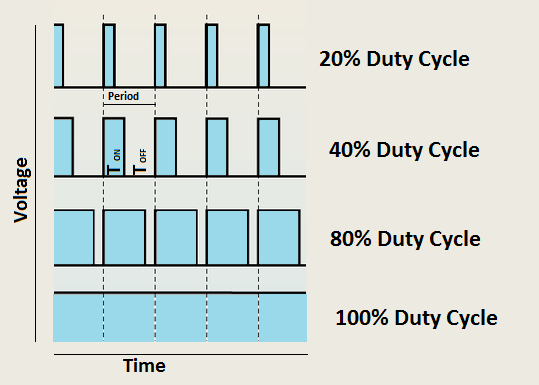
\includegraphics[keepaspectratio=true, width=0.5\textwidth]
    	{img/pwm.png}
    \fonte{https://create.arduino.cc/projecthub/muhammad-aqib/arduino-pwm-tutorial-ae9d71}
    \label{fig:pwm}
\end{figure}

\begin{figure}[H]
    \centering
    \caption{Microcontrolador ESP32}
    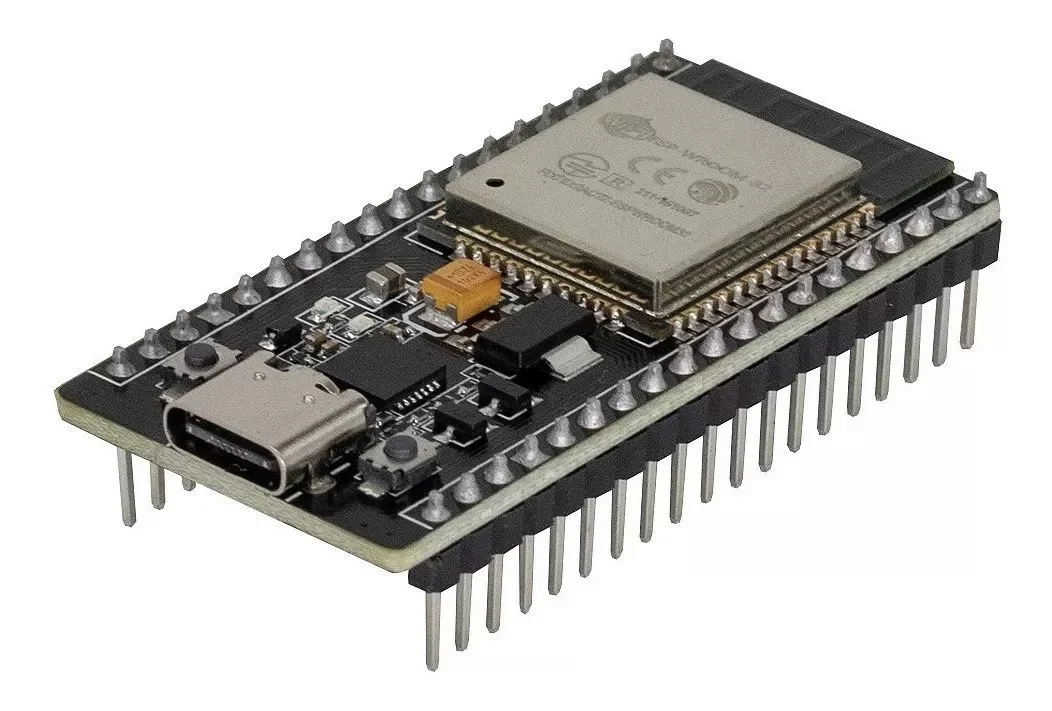
\includegraphics[keepaspectratio=true, width=0.5\textwidth]
    	{img/foto-esp32.png}
    \fonte{https://www.robobuilders.com.br/nodemcu-esp32-38-pinos-devkit}
    \label{fig:fotoESP32}
\end{figure}

\subsection[Placa de Controle]{Placa de Controle}
\label{sub:placaControle}

Para controlar os motores do manipulador, é necessário o uso de uma placa de controle para converter os sinais de baixa potência provenientes do microcontrolador em sinais de maior potência que movimentam as juntas do manipulador robótico.
Essa placa é alimentada com 12v e recebe os sinais digitais de direção e de \textit{PWM} do ESP32 e movimenta os motores de acordo.

Para obter essa funcionalidade, foi decidido utilizar módulos de ponte H, que são circuitos integrados (CI) utilizados para aplicar uma tensão variável a um componente através de um sinal de \textit{PWM}.
Eles também permitem alterar a direção em que a corrente é aplicada no componente, o que possibilita inverter o sentido de rotação de um motor \cite{h_bridge}.
A figura \ref{fig:ponteH} apresenta um módulo de ponte H disponível no mercado, que utiliza o CI L298N.

\begin{figure}[H]
    \centering
    \caption{Módulo de ponte H}
    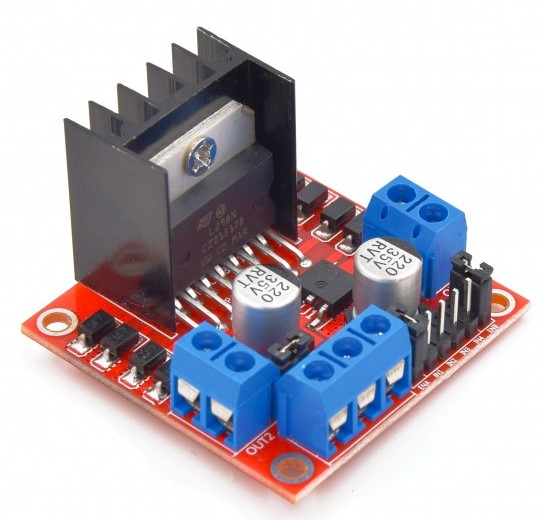
\includegraphics[keepaspectratio=true, width=0.5\textwidth]
    	{img/ponte-h.jpg}
    \fonte{https://www.smart-prototyping.com/L298N-Dual-H-bridge-Motor-Driver-Board}
    \label{fig:ponteH}
\end{figure}

\subsection[Computador]{Computador}
\label{sub:computador}

Para gerenciar o jogo de xadrez, foi decidido utilizar um computador.
Ele é responsável por implementar a lógica do jogo de xadrez e enviar sinais de controle para o ESP32, que por sua vez controla o manipulador robótico.

Para realizar a comunicação entre o computador e o ESP32, pode ser feito uso do protocolo serial, através de um cabo USB.
Através dele o computador envia sinais indicando para qual casa do tabuleiro o manipulador deve mover, e quando ele deve pegar ou soltar uma peça.
Por outro lado, o ESP32 envia sinais indicando quando o movimento foi finalizado e, no modo manual, qual movimento o jogador deseja realizar.

Para implementar as regras do jogo, é necessário desenvoler um software para interagir com uma \textit{engine} de xadrez.
Através dele, é possível verificar os movimentos válidos e identificar quando o jogo terminou.
Além disso, ele também é responsável por converter um movimento em uma sequência de comandos que devem ser enviados ao ESP32.

\section[Projeto do sistema]{Projeto do sistema}
\label{sec:projetoSistema}

Após a definição de todos os equipamentos a serem utilizados, foi feito o projeto do sistema,
indicando como os componentes devem ser conectados.

A manete deve ser alimentada com 3.3V e ser conectada ao ESP32 para permitir a leitura dos sinais de entrada.
Essa conexão é realizada com 10 cabos, sendo 5 para cada \textit{joystick} com seu respectivo botão.

A placa de controle deve ser alimentada com 12V e também deve ser conectada ao ESP32 para receber os sinais de controle.
Essa conexão é realizada com 10 cabos, 2 para o controle de cada junta do manipulador robótico.
Essa placa também deve ser conectada aos motores do manipulador robótico, também com 10 cabos, 2 para cada junta.

O manipulador robótico deve ser conectado ao ESP32 para o envio dos sinais de posição de cada junta.
Essa conexão é realizada com 5 cabos, um para cada junta.

Por fim, o ESP32 deve ser alimentado com 3.3V e deve ser conectado a um computador para a implementação da lógica do jogo.

A montagem do sistema é mostrada na Figura \ref{fig:montagemSistema}.

\begin{figure}[H]
    \centering
    \caption{Montagem do sistema}
    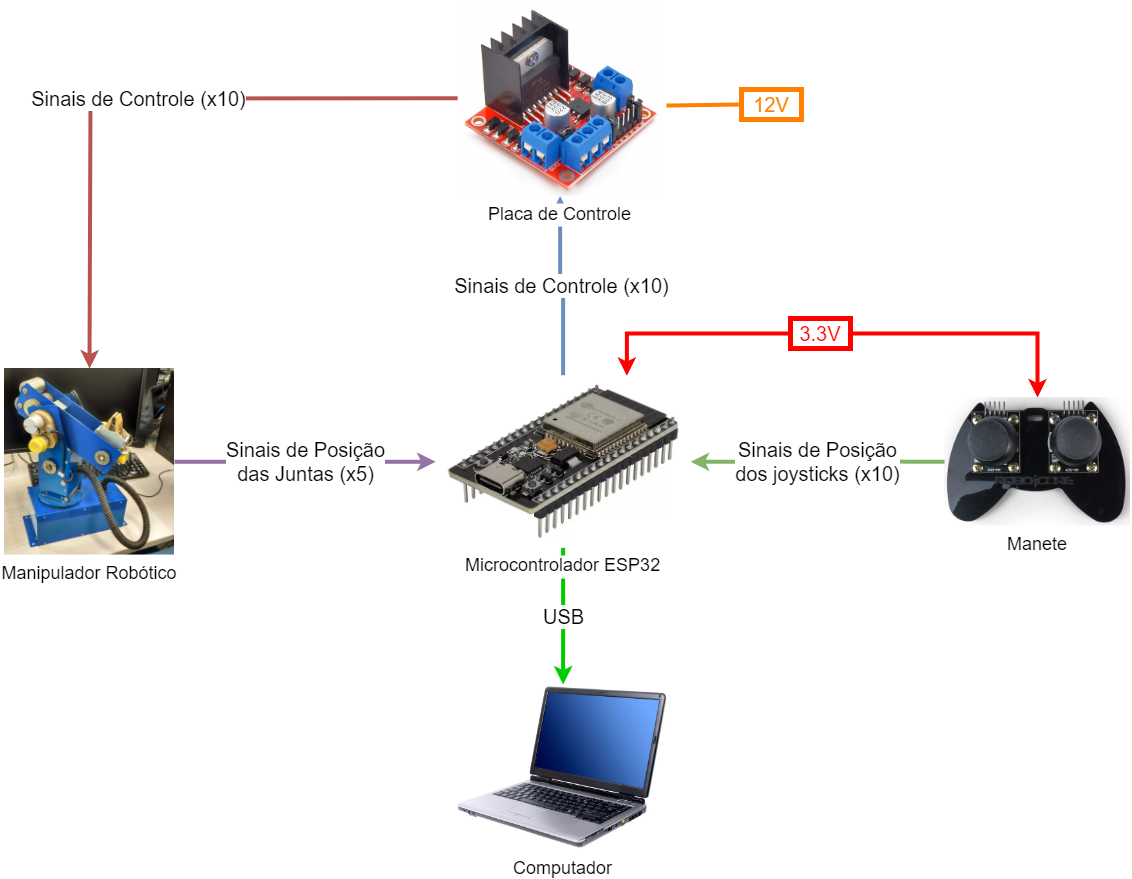
\includegraphics[keepaspectratio=true, width=0.8\textwidth]
    	{img/projeto-sistema.png}
    \fonte{Do próprio autor}
    \label{fig:montagemSistema}
\end{figure}


